\begin{infocard}{Proporcionalidad directa}
    Colocaremos en una tabla los 3 datos (a los que llamamos $a$, $b$ y $c$) y la incógnita, es decir, el dato que queremos averiguar (que llamaremos $x$). Después, aplicaremos la siguiente fórmula:
    \begin{figure}[H]
        \centering
        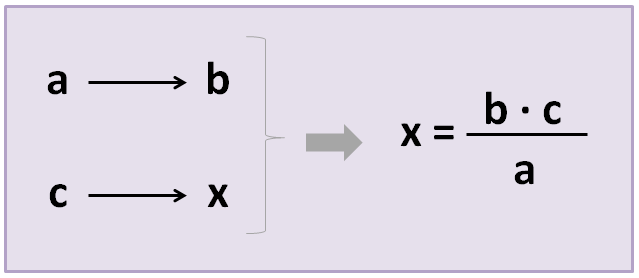
\includegraphics[width=.75\linewidth]{../images/formula-regla-de-3-img1}
        \caption{Solución de una relación proporcional \textbf{directa} por medio de la regla de 3}
        \label{fig:}
    \end{figure}
\end{infocard}
